\newpage
\section{Tuesday, February 25, 2020}


\subsection{Prefix Codes}

One particular class of encoding schemes are \vocab{prefix codes}. A prefix code for a set $S$ of letters is a function $\gamma$ that maps each letter $x\in S$ to some sequence of zeros and ones in such a way that for any $x, y \in S$ with $x \neq y$, the sequence $\gamma(x)$ is not a prefix of the sequence $\gamma(y)$. Why do many encoding schemes fall into this class? Because it removes ambiguity: --- if there exists a pair of letters where the bit string that encodes one letter is a prefix of the bit string that encodes the other, then there might be multiple interpretations of the same string.  \\

The ambiguity of encoding schemes that aren't prefix codes is demonstrated through the following example:

\begin{example}
[Ambiguity Morse Code] In Morse code, we typically encode letters with dashes and dots. For our purpose, we can think of dots and dashes as zeros and ones. Suppose $e$ maps to $0$ (a single dot), $t$ maps to $1$, and $a$ maps to $01$. Then the string $0101$ can have several interpretations: it can mean $eta, aa, etet$, or $aet$. If the morse code were a prefix code, then this problem wouldn't be present.
\end{example}


Now, here's an example illustrating the ease of using a prefix code:

\begin{example}
[Prefix Code Example] Suppose we have a set $S = \{a, b, c, d, e\}$ with the encoding $\gamma(a) = 11, \gamma(b) = 01, \gamma(c) = 001, \gamma(d) = 10, \gamma(e) = 000$. This defines a prefix code since no encoding is a prefix of any other. The string $cecab$ is encoded as $0010000011101$, and a recipient of this message can decipher this message to our single unique message.
\end{example}

In order to efficiently decipher a prefix code, we need an effective way to represent the prefix code so that we can easily pick off the codeword. This is typically done with a binary tree in which the leaves of the tree store the characters of our alphabet. How does this work? We interpret the binary codeword for a character as a simple path from the root to that character; the bit $0$ tells us to go to the left child, whereas the bit $1$ tells us to go to the right child. \\

The following binary search tree illustrates a prefix code representation:

\begin{figure}[h]
\centering
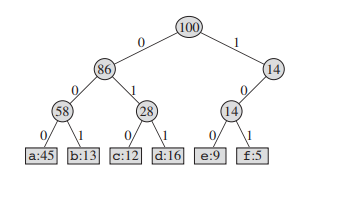
\includegraphics[scale=1]{media/prefix}
\caption{Prefix Code Representation}
\end{figure}

If we had the sequence $001011101$, then we could start at the root, and we'd scan our sequence from left to right. First, we counter two zeros, so we go to the left twice. At this point, we'd be at the vertex labelled $58$. Next, we encounter a $1$, so we go to the right. Thus, we obtain the character $b$. Next, we start at the root again, and we follow our procedure again. The next character that we decipher is $d$. This process continues until there are no more bits to process. \\


Given a tree $T$ corresponding to a prefix code, we can now easily compute the number of bits required to encode a file. In particular, for each character $c$ in our alphabet $S$, we can let $\verb!freq[c]!$ denote the frequency of $c$ in our file. Moreover, we can let $d_{T}(c)$ denote the depth of $c$'s leaf in the tree. With this notation, the number of bits required to encode a file is given by 
\[
\sum_{c \in S} \verb!freq[c]! \cdot d_{T}(c).
\]

We call this the \vocab{cost} of the tree $T$. 

\subsubsection{Constructing a Huffman code}

Now that we've introduced prefix codes, we'll talk about an optimal prefix code known as a \vocab{Huffman code}, whose tree representation has minimum cost. The algorithm constructing the tree is presented below: \\

\newpage

\vspace{1em}
\begin{center}
\line(1,0){400}
\end{center}

\begin{allintypewriter}
\# Input: A set C representing the set of all possible characters that 

\# might appear in our text, and an array freq[] in which freq[k] represents 

\# the frequency of the character k in our text.

\# Output: The root of a binary representing our encoding minimum cost.

\hspace{0cm}

HUFFMAN(C, freq) \string{

\hspace{0.5cm} let Q be a minimum priority queue

\hspace{0.5cm} for each element c in C \string{ enqueue c into Q \string }

\hspace{0cm}

\hspace{0.5cm} for i = 1 to n - 1 \string{

\hspace{1cm} let z be a new node

\hspace{1cm} x = EXTRACT-MIN(Q)

\hspace{1cm} y = EXTRACT-MIN(Q)

\hspace{1cm} z.left = x

\hspace{1cm} z.right = y

\hspace{1cm} \verb!freq[z] = freq[x] + freq[y]!

\hspace{1cm} insert z into Q.

\hspace{0.5cm} \string}

\hspace{0.5cm} return EXTRACT-MIN(Q) /* Return the root of the tree. */

\string}

\begin{center}
\line(1,0){400}
\end{center}
\end{allintypewriter}

How does this algorithm work?

\begin{enumerate}
    \item Firstly, we enqueue all of the characters in $C$ into our minimum priorty queue $Q$.
    \item The for-loop repeatedly extracts the two vertices with the lowest frequency and replaces them in the queue with a new node representing their ``merger" (parent). The frequency of $z$ is the sum of the frequencies of $x$ and $y$.
    \item After $n - 1$ merges, there's only one node left in the queue, which is the root of the code tree.
\end{enumerate}

If we're using a binary heap, then the algorithm runs in $\mathcal{O}(n\log(n))$ time since we perform $\mathcal{O}(n)$ calls to \verb!EXTRACT-MIN!, which is an $\mathcal{O}(\log(n))$ operation.


While we won't show it, it can be shown that this construction of a tree is optimal. This procedure counts as a greedy algorithm since, at each step, we greedily extract the characters with the lowest frequency.


\subsection{Matrix Multiplication}

The next problem we'll discuss is stated as follows:

\begin{quote}
    Given two $n\times n$ matrices $A$ and $B$, compute the $n \times n$ matrix $C$ whose $(i, j)^{\text{th}}$ entry is defined by $c_{ij} = \sum_{k=1}^{n}a_{ik} b_{kj}$. In other words, we want to compute the product $C = AB$. 
\end{quote}

The brute force solution is $\mathcal{O}(n^3)$. In this algorithm, we just use three loops, and we compute each value $c_{ij}$ in $C$ as the summation provided in the problem statement. Of course, we want to do better. \\

Another idea is to perform a divide-and-conquer technique on the matrix. In particular, we can divide the matrix into four submatrices (top left corner, top right corner, bottom left corner, bottom right corner), and we can calculate the products recursively. The time complexity of this algorithm is given by the recurrence $T(n) = 8T(n/2) + \mathcal{O}(n^2)$. Unfortunately, by Master's Theorem, we know that the solution to this recurrence will be $\mathcal{O}(n^3)$, which isn't any better. 